\documentclass[11pt,a4paper]{article}

\usepackage{amsmath} %for mathemathic formulas
\usepackage{amssymb}
\usepackage[ngerman]{babel} %for the german language by the spellling reform (without the package the date would look like April 20, 2020)
\usepackage{enumitem} %for enumeration surrounding 
\usepackage{graphicx} %for pictures
\usepackage{siunitx}
\usepackage{float}

\title{Blatt 10}
\date{\today}
\author{Hannah Rotgeri \and Feline Heinzelmann}

\begin{document}
    \maketitle


	\begin{itemize}
		\item[a)] 
			Teilchen in einem Synchrotron bewegen sich auf einer Kreisbahn
			und erfahren demnach eine Beschleunigung.
			Da beschleunigte Ladungen Photonen emittieren,
			wird Synchrotronstrahlung abgestrahlt.

		\item[b)]
			Das kontinuerliche Spektrum hat ein Maximum bei kleinen Frequenzen und 
			wird durch die kritische Energie in zwei gleichgroße Leistungsintegrale geteilt.

		\item[c)] 
			Das Spekturm eines Undulators entspricht einer Linie bei der fundamentalen Wellenlänge.
			Da in der Realität die Fouriertransformation nur über einen begrenzeten Zeitraum stattfindet,
			hat die Linie eine endldliche Breite.
			Ist K > 1 sieht der Beobachter auch die ungeraden Harmonischen.
			Bei einem Beobachtungswinkel $\theta$ sieht der Beobachter auch die geraden Harmonischen.
			\begin{equation}
				\lambda = \frac{\lambda_u}{2 \gamma ²} (1 + K²/2 + \gamma² \theta²).
			\end{equation}

		\item[d)]
			Ein Wiggler ist hat ein größeres K und somit im Spektrum höhere harmonische der Grundfrequenz.
			Die Brillanz ist beim Wiggler proportional zu N und beim Undulator proportional zu N².
			Ein Wellenlängenschieber ist ein supraleitender Dipolmagnet dessen hohes Feld das Spektrum zu kürzeren Wellenlängern verschiebt.
			Wird ein "normaler" Dipolmagnet durch einen supraleitenden ersetzt· wird dieser als superbend bezeichnet.

		\item[e)]
			FEL hat kürzere Pulse, gereinere Emittanz und kohärente Abstrahlung.
		
		\item[f)]
			Eine Energieabweichung bewirkt eine Änderung der Phase und umgekehrt.
			Die Pondomotorische Phase gibt den Phasenunterschied zwischen Elektronenpaket und Laserfeld an.
			Ist die Pondomotorische Phase konstant, gibt es einen kontinuierlichen Enrgieaustausch.
		
		\item[g)]
			Beim high-gain FEL werden die zwei Gleichungen durch eine dritte ergänzt,
			denn die Amplitude es elektrischen Feldes ändert sich.
			Die Energieänderung ist proportional zum bunching-Faktor.
			Dieser ist ein Maß dafür, ob die Elektronen gleichverteilt sind,
			oder bei einer bestimmten Phase eine höhere Elektronendichte ist.
		
		\item[h)]
			Beim SASE-FEL entsteht im ersten Teil eines Undulators durch spontane Strahlung ein Strahlungspuls,
			der im zweiten Teil verstärkt wird. 
			Dabei unterliegt die spektrale Verteilung statistischen Schwankungen.
			Allerdings ist der Prozess auch einfach und robust.
			Beim seeding, wird ein externer Puls verstärkt.
			Ein Vorteil ist neben der Kontrollierbarkteit, 
			dass der Puls automatisch mit einer externen Quelle synchronisiet ist (Anrege-Abfrage-Experimente).
			Es kann entweder mit der FEL-Wellenlänge geseedet werden, oder mit einer längeren Wellenlänge.
		
		\item[i)]
			Für SASE wird eine kleine Emittanz und ein hoher Spitzenstrom benötigt.
			Die Länge der Pakete wird durch das Gleichgewicht zwischen Aufheizen und Dämpfung durch die Synchrotronstrahlung bestimmt.
		
		\item[j)]
			
		
		\item[k)]
		
		
		\item[l)]
			Kollektive Phänomene treten durch Wechselwirkung der Teilchen untereinander auf.
			Bei Störungen durch optische Resonanzen, kommt es zu einem verstärkenden Effekt, 
			da die gleichen Teilschen mehrfach mit einer externen Störung ineragieren.
			Bei kollektiven Phänomenen interagieren entweder unteschiediche Teilchen miteinander 
			oder das selbe Teilchen (bzw. Teilchenpaket) mit einem durch dieses Teilchen erzeugten Feld.

		\item[m)]
			\begin{figure}[H]
				\centering
				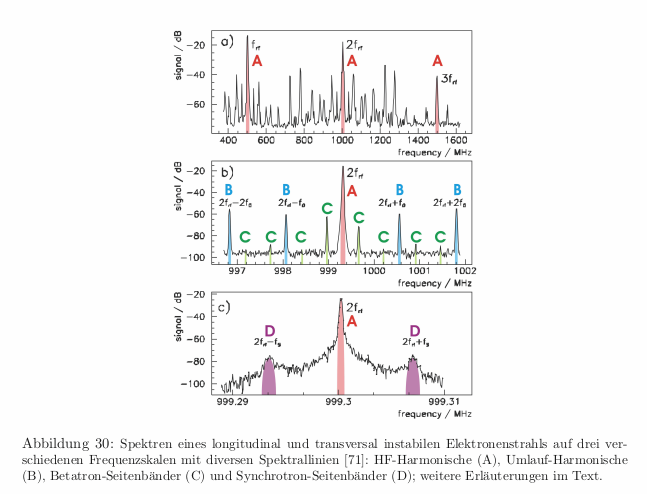
\includegraphics[width=\textwidth]{sprektrum.png}
			\end{figure}
		
		\item[n)]
			Wake-Felder sind Felder, die die Strahlteilchen selber erzeugen.
			Die Strahlteilchen erzeugen in der Vakuumkammer ein elektrisches Feld,
			welches sich auf Grund der endlichen Leitfähigkeit nicht instantan abbauen kann.
			Im Frequenzraum ist die Impedanz das analogon zum ohmschen Wiederstand.
		
		\item[o)]   
		
		
		\item[p)]      
			\begin{itemize}
				\item Einteilchen-Modell (Teilchenpaket als ein Makroteilchen): multi bunch- Instabilitäten
				\item Zweiteilchen-Modell: head-teil-Instabilität
				\item kontinuerliche Ladungsverteilung: kopliziertere Moden innerhalb eines Pakets simulieren
			\end{itemize}


	\end{itemize}

\end{document}